%compile with pdflatex on papeeria

\documentclass[a4paper,12pt]{article}
\usepackage{fancyhdr}
\usepackage{fancyheadings}
\usepackage[ngerman,german]{babel}
\usepackage{german}
\usepackage[utf8]{inputenc}
%\usepackage[latin1]{inputenc}
\usepackage[active]{srcltx}
%\usepackage{algorithm}
%\usepackage[noend]{algorithmic}
\usepackage{amsmath}
\usepackage{amssymb}
\usepackage{amsthm}
\usepackage{bbm}
\usepackage{enumerate}
\usepackage{graphicx}
\usepackage{ifthen}
\usepackage{listings}
\usepackage{enumitem}
%\usepackage{struktex}
\usepackage{hyperref}
\usepackage{tikz}
\usepackage{float}
\usepackage{subcaption}
\captionsetup{compatibility=false}
\captionsetup[subfigure]{labelformat=empty}

\usepackage{pgfplots}
\pgfplotsset{compat=1.15}
\usepackage{mathrsfs}
\usetikzlibrary{arrows}

\definecolor{kolorwykresu}{rgb}{0.07,0.04,0.56}
\definecolor{ccqqqq}{rgb}{0.8,0,0}

\definecolor{qqwuqq}{rgb}{0,0.39215686274509803,0}
\pagenumbering{gobble}

%%%%%%%%%%%%%%%%%%%%%%%%%%%%%%%%%%%%%%%%%%%%%%%%%%%%%%
%%%%%%%%%%%%%% EDIT THIS PART %%%%%%%%%%%%%%%%%%%%%%%%
%%%%%%%%%%%%%%%%%%%%%%%%%%%%%%%%%%%%%%%%%%%%%%%%%%%%%%
\newcommand{\Fach}{1. Klausur aus der Mathematik (A)}
\newcommand{\Name}{}
\newcommand{\datum}{}
\newcommand{\Matrikelnummer}{}
\newcommand{\Semester}{Q11/2}
\newcommand{\Uebungsblatt}{} %  <-- UPDATE ME
%%%%%%%%%%%%%%%%%%%%%%%%%%%%%%%%%%%%%%%%%%%%%%%%%%%%%%
%%%%%%%%%%%%%%%%%%%%%%%%%%%%%%%%%%%%%%%%%%%%%%%%%%%%%%

\setlength{\parindent}{0em}
\topmargin -1.0cm
\oddsidemargin 0cm
\evensidemargin 0cm
\setlength{\textheight}{9.2in}
\setlength{\textwidth}{6.0in}

%%%%%%%%%%%%%%%
%% Aufgaben-COMMAND
\newcommand{\Aufgabe}[1]{
  {
  \vspace*{0.5cm}
  \textsf{\textbf{Aufgabe #1}}
  \vspace*{0.2cm}
  
  }
}
%%%%%%%%%%%%%%
\hypersetup{
    pdftitle={\Fach{}: Übungsblatt \Uebungsblatt{}},
    pdfauthor={\Name},
    pdfborder={0 0 0}
}

\lstset{ %
language=java,
basicstyle=\footnotesize\tt,
showtabs=false,
tabsize=2,
captionpos=b,
breaklines=true,
extendedchars=true,
showstringspaces=false,
flexiblecolumns=true,
}

\title{Übungsblatt \Uebungsblatt{}}
\author{\Name{}}

\begin{document}
\thispagestyle{fancy}
%\lhead{\sf \large \Fach{} \\ %\small \Name{} - \Matrikelnummer{}
\lhead{\sf \large \Fach{} %\small \Name{} - \Matrikelnummer{}
}
\rhead{\sf \Semester{}   \datum{}}
%\rhead{\sf \Semester{} }
\vspace*{0.2cm}
%\begin{center}
%%\LARGE \sf \textbf{Übungsblatt \Uebungsblatt{}}
%\end{center}
%\vspace*{0.2cm}

%%%%%%%%%%%%%%%%%%%%%%%%%%%%%%%%%%%%%%%%%%%%%%%%%%%%%%
%% Insert your solutions here %%%%%%%%%%%%%%%%%%%%%%%%
%%%%%%%%%%%%%%%%%%%%%%%%%%%%%%%%%%%%%%%%%%%%%%%%%%%%%%

  Name: \underline{\hspace{7cm}}
  \hfill
  Datum: \underline{\hspace{4cm}}

%\vspace{0,5cm}Die Rechenwege müssen nachvollziehbar sein!
%
%\vspace{0,5cm} {TEIL A} - ohne Hilfsmittel - Bearbeitungszeit 30 Minuten
%\vspace {0,2cm}
% 
%GEOMETRIE

\Aufgabe{1} 


%\begin{tabular}{|p{0.18cm}|m{0.18cm}|b{0.18cm}|l|}
%\hline
%a\newline a & b\newline b & c\newline c\newline c& d \\
%\hline
%\end{tabular}


\begin{enumerate}[label={\alph*)}]
\item Geben Sie den Term einer Funktion $f$ an, deren Steigung immer konstant ist.
\item Beschreiben Sie in einem Satz die Bedeutung der lokalen Änderungsrate in dem untensthenden Beispiel. \\

  \begin{tabular}{|c|c|}
    \hline
    Größe F (Einheit von F) & Lokale Änderungsrate der Größe F \\[2.5ex] \hline 
    Länge einer Pflanze (cm) & ? \\[2.5ex] \hline
  \end{tabular}
  

\item 
  Gegeben ist die Funktion $f(x) = \ln(6-x)$ \\
Ermitteln Sie auf nachvollziehbare Weise den maximalen Definitionsbereich $D_f$ und weisen Sie nach, dass die Funktion $f(x)$ keine Extrema besitzt!


\item Eine Tangente berührt den Graphen der Funktion $f: x \rightarrow 0,5x^2 - 11$
an der Stelle $x_0 = 4$. Bestimmen Sie die Gleichung der Normalen, welche auf dieser Tangente senkrecht steht.
\end{enumerate}
\begin{flushright}8 BE \end{flushright}

\Aufgabe{2:} 
Gegeben ist die Funktion $f: x \rightarrow \frac{x^2}{9-3x}$
\begin{enumerate}[label={\alph*)}]
  \item Geben Sie die maximale Definitionsmenge $D_f$ und die Nullstellen von $f$ an.\\
Die Funktion $f$ lässt sich auch in der Form
    $f(x) = - \frac{1}{3}x - 1 + \frac{3}{3-x}$ 
darstellen (kein Nachweis erforderlich).


\item Untersuchen Sie das Verhalten an den Rändern der Definitionsmenge und geben Sie die Gleichungen aller Asymptoten des Graphen an!
\item Ermitteln Sie das Monotonieverhalten und die Lage und Art der Extrema der Funktion.\\
 \lbrack Zur Kontrolle: $f'(x) = (-3x^2+18x) / (9-3x)^2$\rbrack

\marginpar{
  \begin{center}
Platzbedarf:
7\\
8 11\\
8\\
  \end{center}
}
\item Skizzieren Sie den Graphen von $f$ unter Verwendung der bisherigen Ergebnisse.

\end{enumerate}
\begin{flushright}17 BE \end{flushright}

  \newpage
\Aufgabe{3:}

Die normale Körpertemperatur eines gesunden Menschen liegt bei 36,5°C. Die Funktion $f$ mit
\[ f(x)=x\cdot{e} ^ {-0,1x} +36,5 \]

beschreibt modellhaft den Verlauf einer Fieberkurve bei einem Erkrankten. Dabei ist $x$ die Zeit in Stunden nach Ausbruch der Krankheit und $f(x)$ die Körpertemperatur in Grad Celsius. Der Graph der Funktion ist in der Abbildung dargestellt.


\begin{center}
  \begin{tikzpicture}[scale=1.5]

  \begin{axis}[
    unit vector ratio=1 1,
    axis x line=center,
    axis y line=center,
    %extra x tick style={tick style={very thick}}
    xtick={-5,0,5,...,45},
    ytick={0,5,...,45},
    ticklabel style = {font=\scriptsize},
    ticklabel style={fill=white},
    %extra x ticks={0},
    %extra y ticks={0},
    %extra y tick style={anchor=south west},
    %extra x tick style={anchor=east},
    %xticklabel style={anchor=south west},
    %minor x tick num=1,
    %minor y tick num=1,
    %minor tick num = 1,
    %x=1cm,    %größe der kästchen in x-richtung
    %y=1cm,    %größe der kästchen in y-richtung
    xlabel={$x$},
    ylabel={$y$},
    %grid=both,
    grid=major, grid style={gray!30},
    grid=minor, grid style={gray!30},
    ymajorgrids=true,
    xmajorgrids=true,
    %extra x ticks=0,
    %extra y ticks=0,
    %extra tick style={tick style={draw=none}},
    %extra y tick style={
    % tick label style={
    % anchor=south east}},
    %extra x tick labels=$0$,
    %extra x tick style={
    % tick label style={
    % anchor=north west}},
    xlabel style={above left},
    ylabel style={below right},
    axis line style = thick,
    xmin=-9,
    xmax=48,
    ymin=-5,
    ymax=42]
      \draw[domain=-10:50, smooth, variable=\x, red] plot ({\x}, {\x*e^(-0.1*\x)+36.5});

    \draw[color=red] (-9,18) node[anchor=north west] {$f$};
    \draw[color=black, yshift=0.05cm, xshift=-0.1cm, font=\scriptsize] (0,0) node[anchor=north west] {$0$};
    \draw[color=black, yshift=-0.08cm, xshift=0.1cm, font=\scriptsize] (0,0) node[anchor=south east] {$0$};
  \end{axis}
\end{tikzpicture}
\end{center}


\begin{enumerate}[label={\alph*)}]
\item Berechnen Sie die maximale Körpertemperatur Tmax sowie den Zeitpunkt xmax, zu dem diese Temperatur erreicht wird. (Antwortsatz!)\\
  (Teilergebnis zur Kontrolle: $f'(x) = (1-0,1x)\cdot{e}^{-0,1x}$)

\item Bestimmen Sie den Zeitpunkt $x_0$, an dem die Körpertemperatur am stärksten abnimmt, und begründen Sie Ihren Rechenweg!


\end{enumerate}

\begin{flushright}9 BE \end{flushright}

\Aufgabe{4:}

\begin{minipage}{0.5\linewidth}
Gegeben ist der Graph einer Funktion $f$:\\

Welcher der folgenden Graphen kann der Graph der Ableitung von $f$ sein?\\

Begründen Sie Ihre Entscheidung anhand von \underline{zwei} verschiedenen Eigenschaften!\\

Geben Sie \underline{jeweils einen} Grund an, warum die übrigen Graphen nicht die Ableitung von $f$ darstellen können!

\end{minipage}\hfil
\begin{minipage}{0.5\linewidth}
    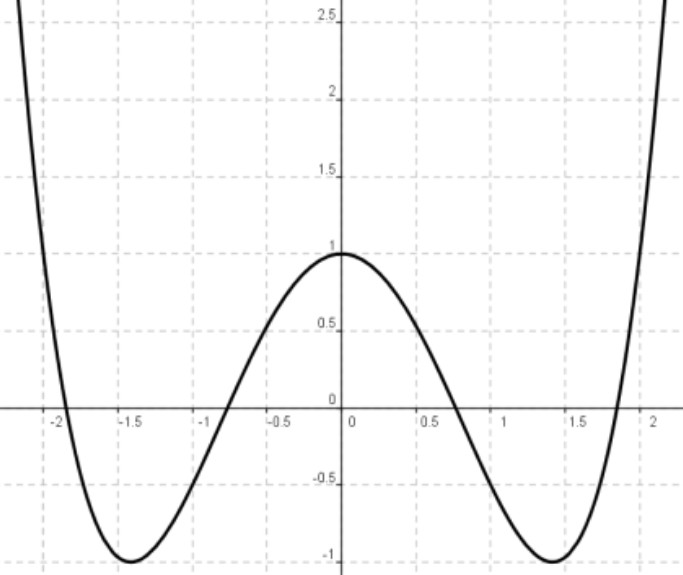
\includegraphics[width=0.8\linewidth]{Q11_210111_4.jpg}
\end{minipage}


%\begin{figure}[h!]
%  \begin{center}
%    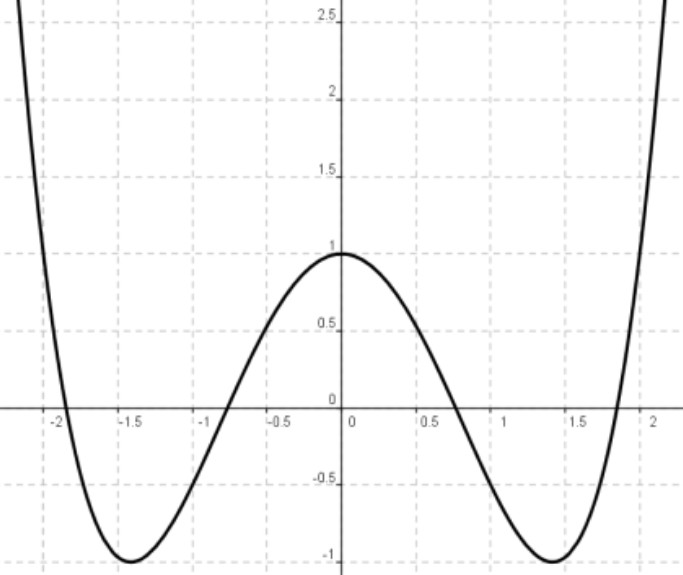
\includegraphics[width=0.7 \linewidth]{Q11_210111_4.jpg}
%  \end{center}
%\end{figure}




\begin{figure}[H]
  \centering

    \subfloat[A]{
          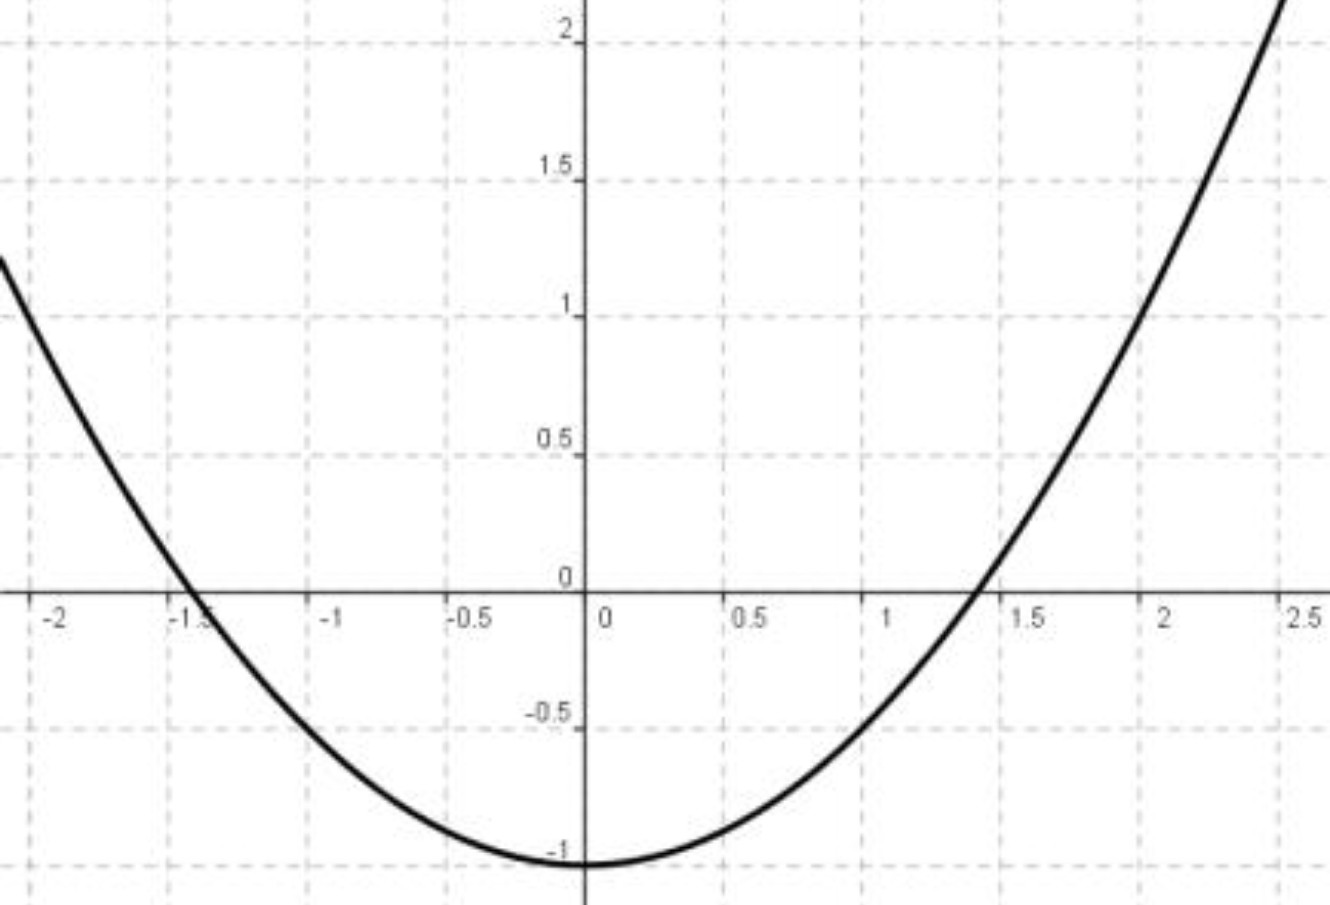
\includegraphics[width=0.3 \linewidth]{Q11_210111_4A.jpg}
        }
    \subfloat[B]{
          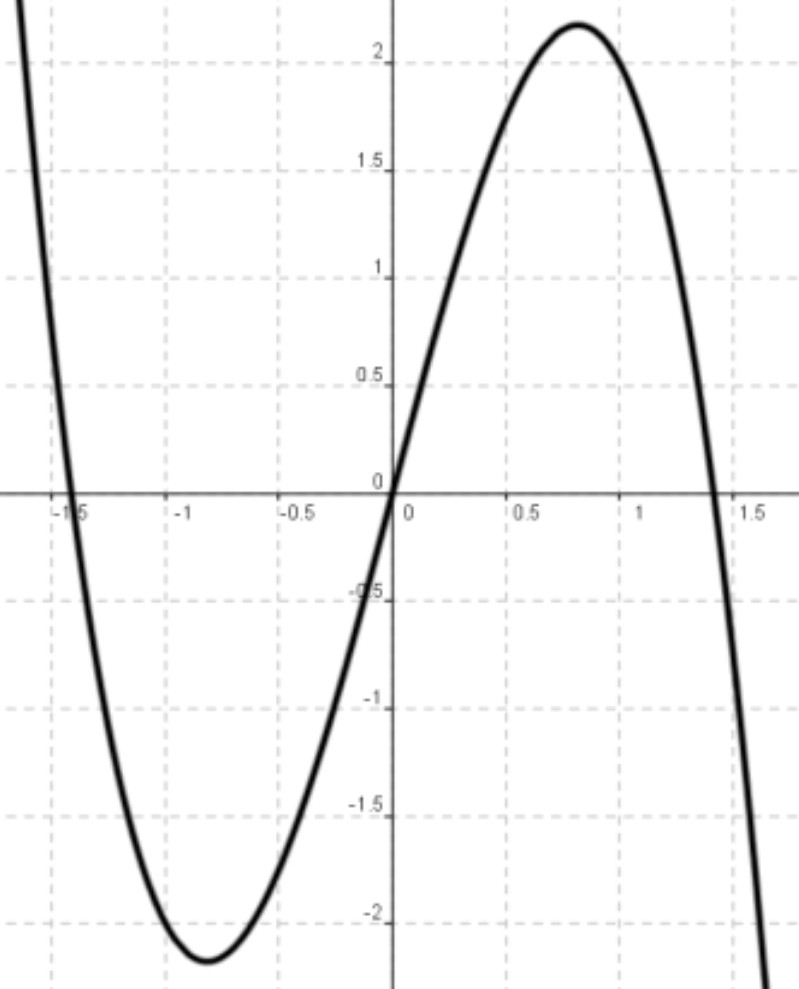
\includegraphics[width=0.3 \linewidth]{Q11_210111_4B.jpg}
    }      %<------------
\end{figure}


\begin{figure}[H]
  \centering

    \subfloat[C]{
          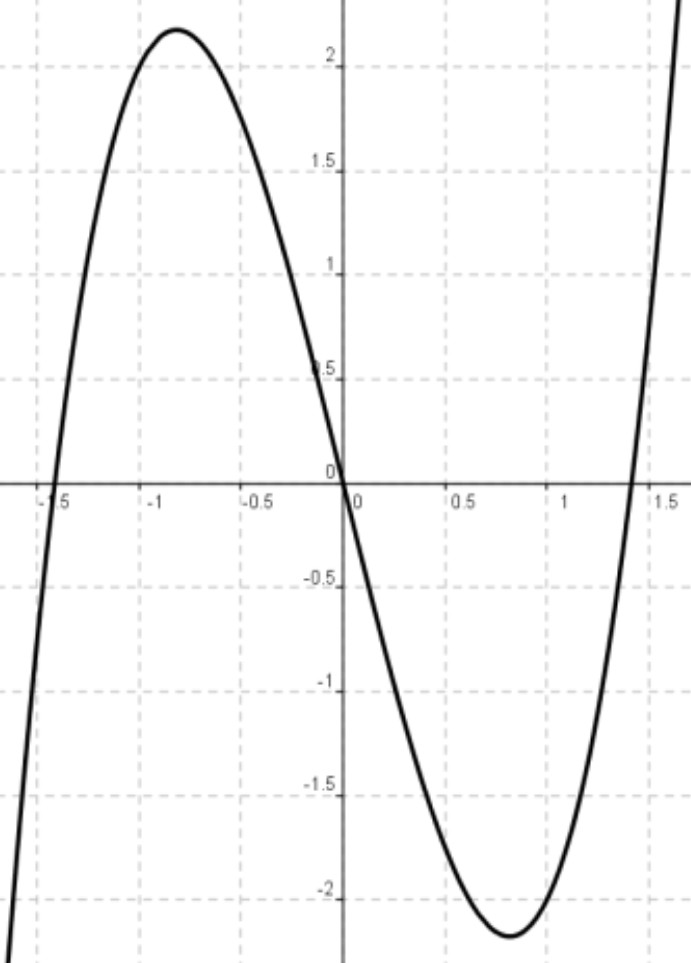
\includegraphics[width=0.3 \linewidth]{Q11_210111_4C.jpg}
    }      
    \subfloat[D]{
          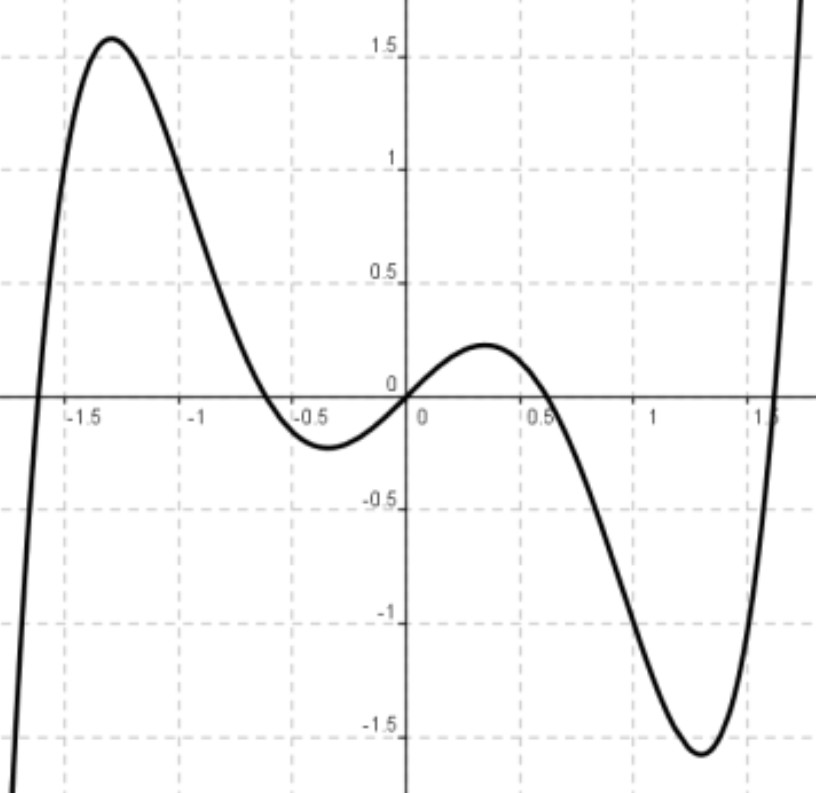
\includegraphics[width=0.3 \linewidth]{Q11_210111_4D.jpg}
    }      
    \subfloat[E]{
          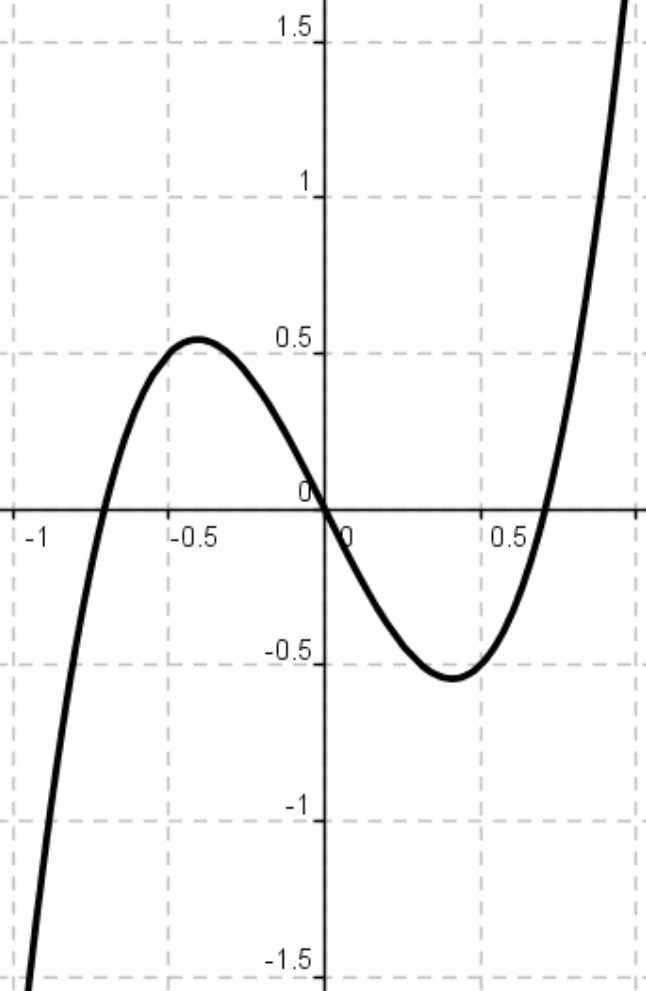
\includegraphics[width=0.3 \linewidth]{Q11_210111_4E.jpg}
    }      
\end{figure}

\begin{flushright}6 BE \end{flushright}
\newpage





\Aufgabe {5:} 

Gegeben sind die Punkte $A(-1|2|1)$, $B(-1|3|3)$, $C(-1|2|5)$ und $D(-1|1|3)$

\begin{enumerate}[label={\alph*)}]
  \item Zeigen Sie, dass das Viereck $ABCD$ eine Raute, aber kein Quadrat ist.
  \item Berechnen Sie den Flächeninhalt der Figur.\\
    {\scriptsize(Haben Sie a) nicht gelöst, dürfen Sie trotzdem davon ausgehen, dass $ABCD$ eine Raute ist.)}
\end{enumerate}

\begin{flushright} 9 BE \end{flushright}
\vspace{0,8cm}


\centerline{Viel Erfolg}
%\enlargethispage{2\baselineskip}

%\addtolength{\voffset}{-2cm}




%\begin{tikzpicture}
%\draw [very thin, black, step=0.5cm] (0,0) grid +(15,18);
%\end{tikzpicture}




%%%%%%%%%%%%%%%%%%%%%%%%%%%%%%%%%%%%%%%%%%%%%%%%%%%%%%
%%%%%%%%%%%%%%%%%%%%%%%%%%%%%%%%%%%%%%%%%%%%%%%%%%%%%%
\end{document}
